\section{Bartosz Warchoł}

\subsection{Na początek szybkie zadanko szachowe}
\begin{figure}[h]
    \centering
    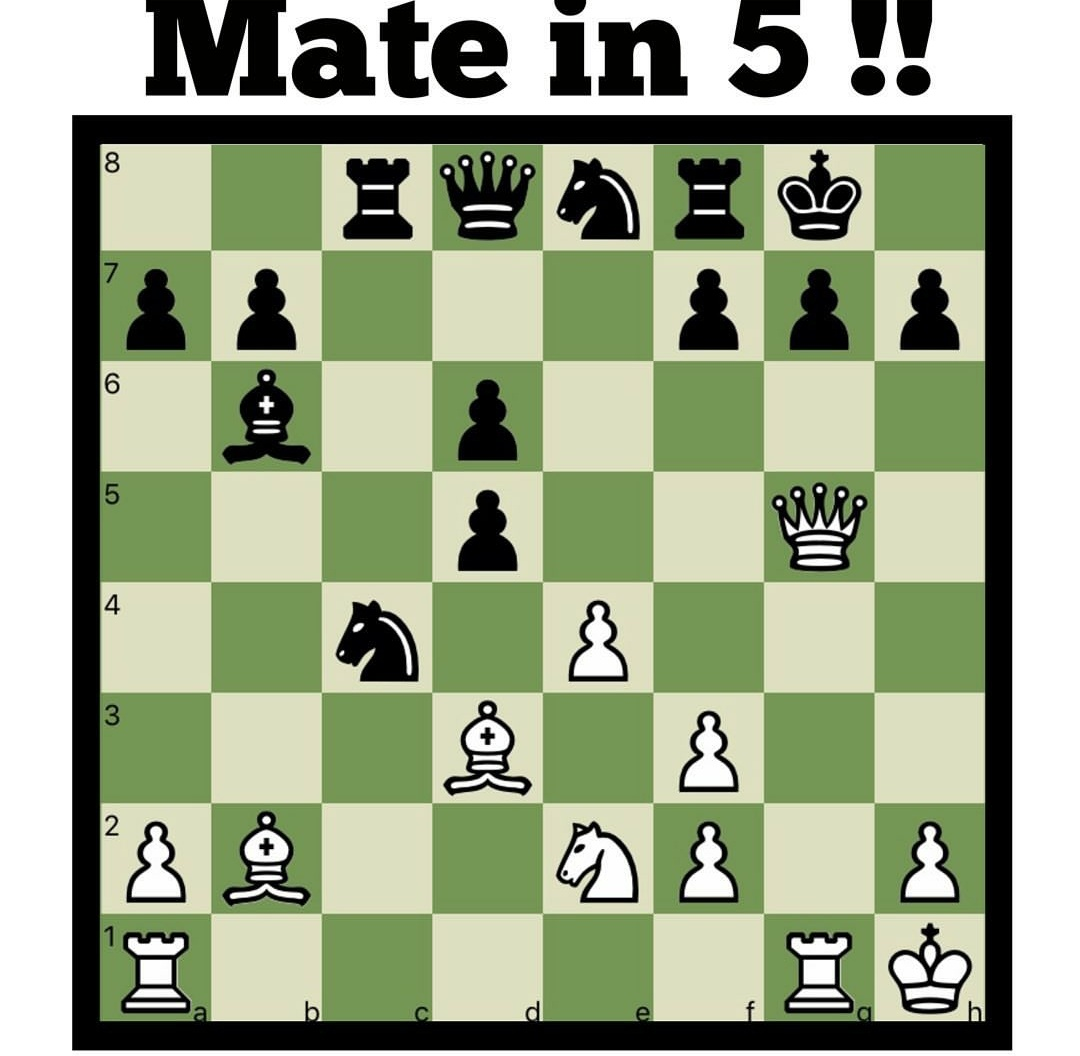
\includegraphics[width=0.75\textwidth]{pictures/tactic.jpg}
    \caption{Jak wyżej - mat w 5}
    \label{chess position}
\end{figure}

\subsection{Delta, delta, delta i nad deltą delta...}

Załóżmy, że mamy wyrażenie:
\begin{equation*}
      \begin{split}
      ax^2 + bx + c = 0\\
      \Delta = b^2 - 4ac\\
      \sqrt{\Delta} = \sqrt{b^2 - 4ac}\\
      x_1 = \frac{-b - \sqrt{\Delta}}{2a}, 
      x_2 = \frac{-b + \sqrt{\Delta}}{2a}
    \end{split}
\end{equation*}

\subsection{Tabela wartości figur szachowych}
\begin{tabular}{ |c|c| } 
        \hline
         wartość & figura \\
         \hline
         \hline
        Pionek & 1 \\
        Skoczek & 3 \\
        Goniec & 3 \\
        Wieża & 5 \\
        Hetman & 9 \\
        Król & none \\
        \hline
    \end{tabular}

\subsection{Ordered list}
\begin{enumerate}
    \item First
    \item Second
    \item Third
\end{enumerate}

\subsection{Unordered list}
\begin{itemize}
    \item First
    \item Second
    \item Third
\end{itemize}

\subsection{The Origin}
\textbf{Chess} is a board game for two players. It is sometimes called \textbf{Western chess} or \textbf{international chess} to distinguish it from related games, such as xiangqi (Chinese chess) and shogi (Japanese chess). The current form of the game \underline{emerged in Spain and the rest of Southern Europe} during the second half of the 15th century \textit{after evolving from chaturanga}, a similar but \textbf{much older game} of Indian origin. Today, chess is one of the world's most popular games, \textbf{\textit{\underline{played by millions}}} of people worldwide. 